\documentclass{article}

\usepackage{graphicx}
\usepackage{tikz}
\usepackage{tikzsymbols}
\usetikzlibrary{calc,patterns,shapes.geometric}
\pagestyle{empty}
\usepackage[margin=0pt]{geometry}
\geometry{papersize={14in,12in}}

\def\centerarc[#1](#2)(#3:#4:#5){\draw[#1] ($(#2)+({#5*cos(#3)},{#5*sin(#3)})$) arc (#3:#4:#5);}

\begin{document}
	\begin{figure}
		\centering
		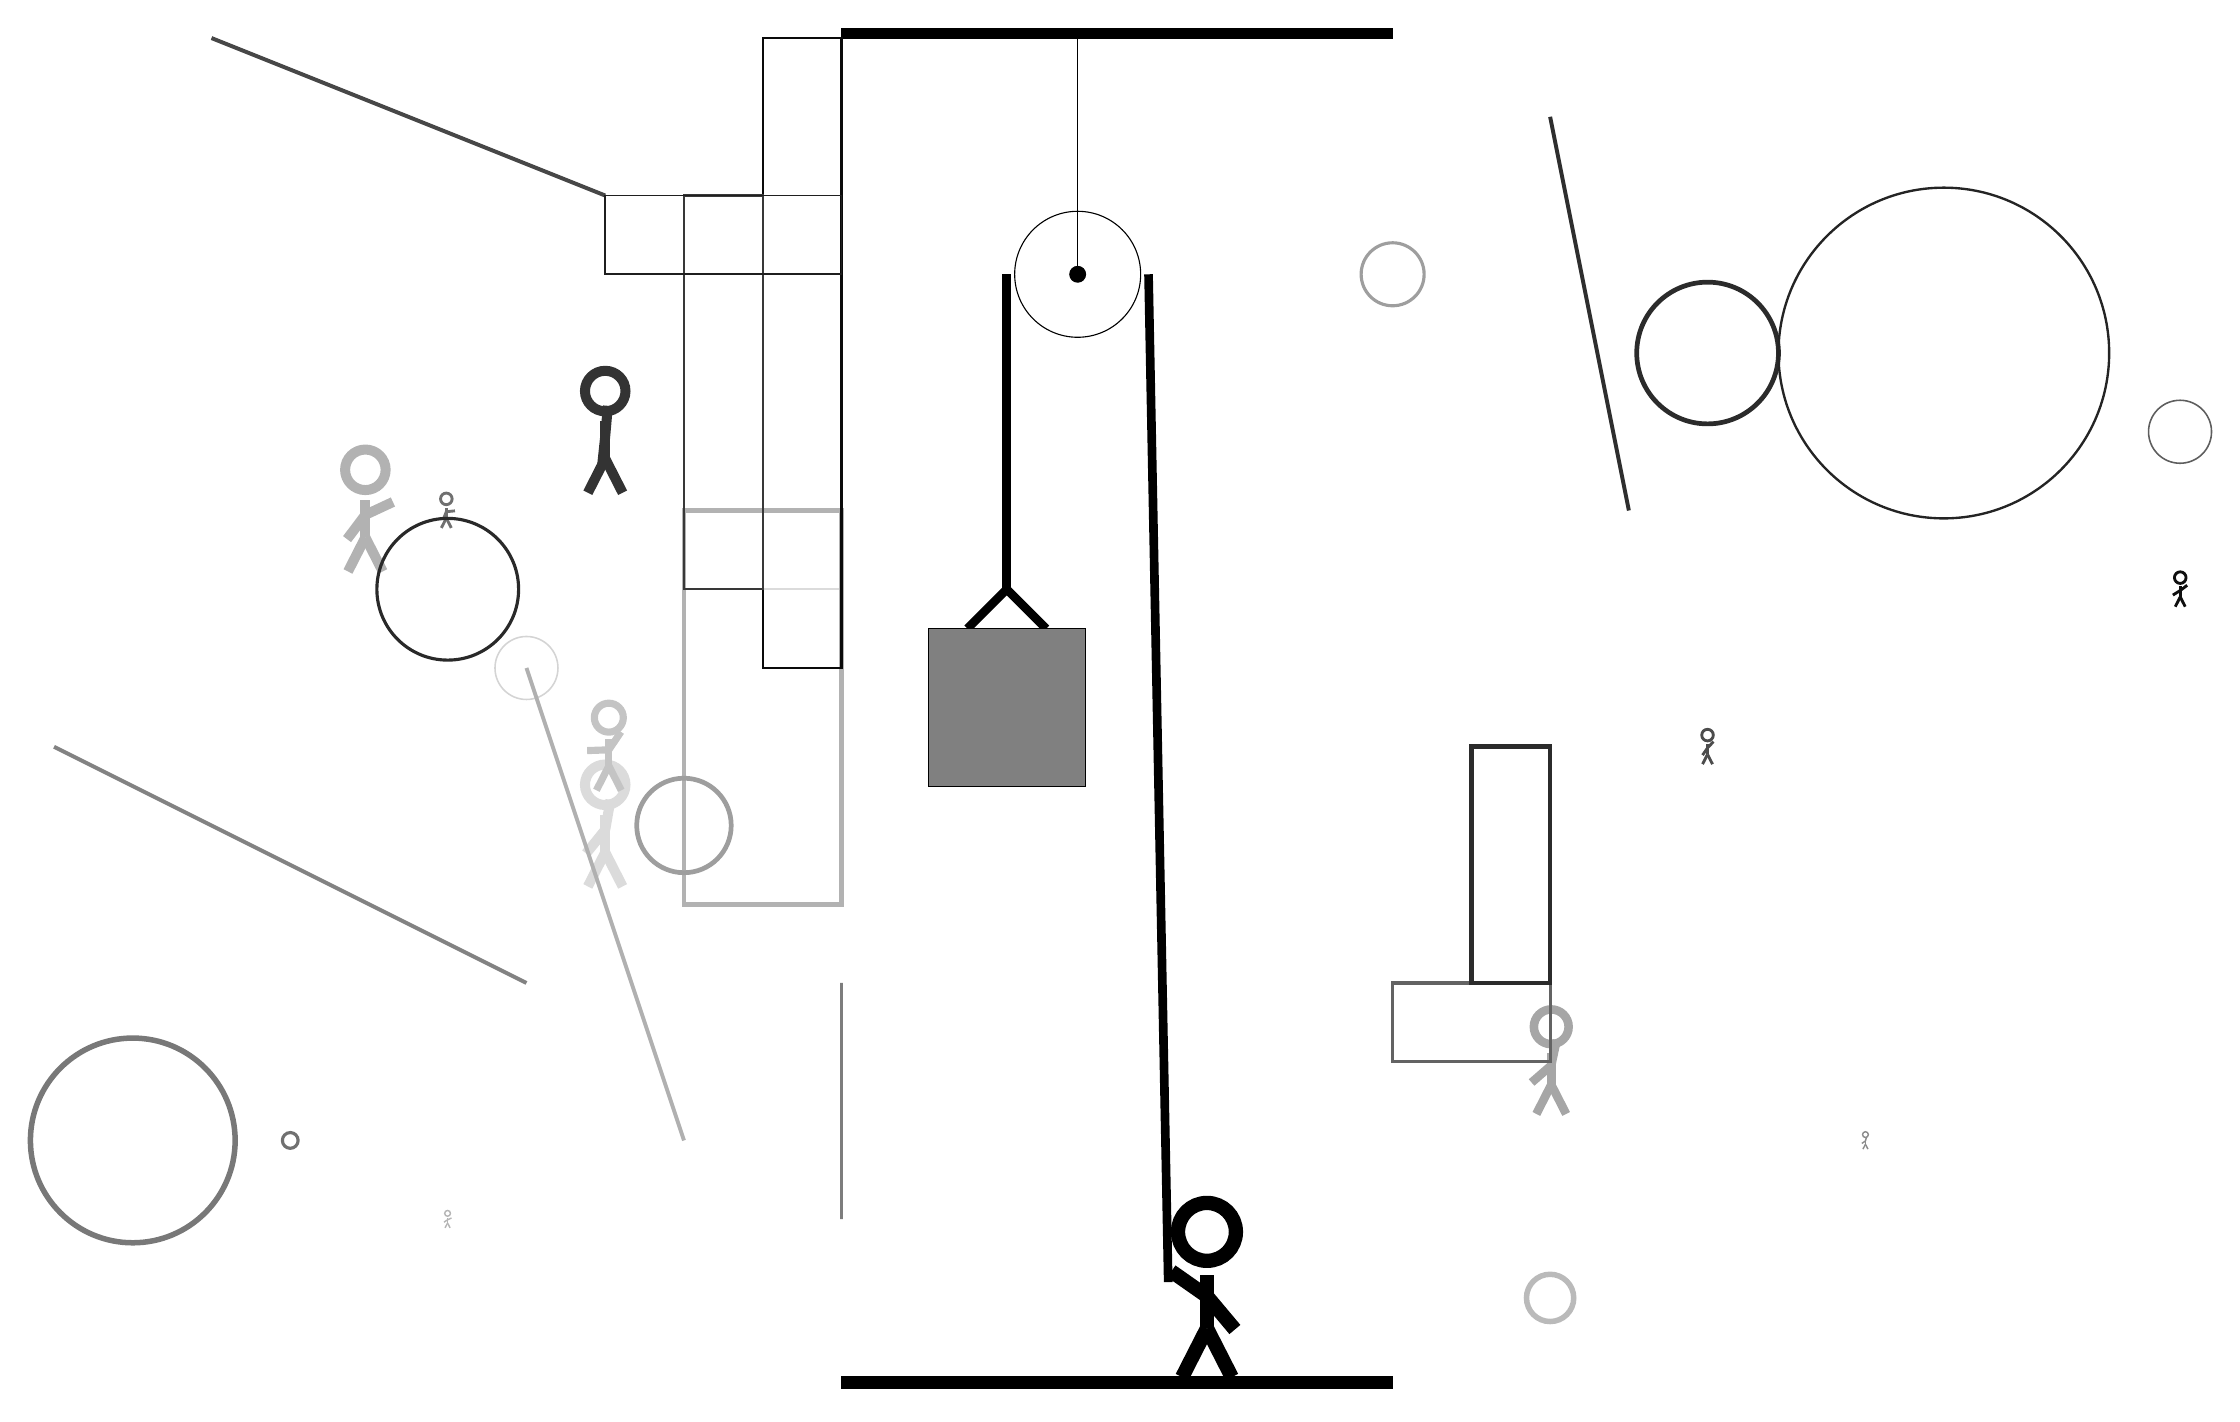
\begin{tikzpicture}
			%%%%% START %%%%%
			
			\draw[fill=black] (-2, 14) rectangle (5, 14.125);
			
			\draw (1, 11) circle (0.8);
			\draw[fill=black] (1, 11) circle (0.1);
			\draw (1, 14) -- (1, 11);
			
			\draw[line width=1.1mm] (-0.4, 6.5) -- (0.1, 7.0) -- (0.6, 6.5);
			\draw[fill=black!50] (-0.9, 6.5) rectangle (1.1, 4.5);
			
			\node[line width=0.3mm, color=black!56] at (-7, 8) {\Strichmaxerl[2][68][6]};
			
			\draw[line width=0.3mm, color=black!14] (-3, 7) rectangle (-2, 6);
			\node[line width=0.5mm, color=black!70] at (9, 5) {\Strichmaxerl[2][55][47]};
			\draw [line width=0.4mm, color=black!56](-9, 0) circle (0.1);
			
			\draw[line width=0.5mm, color=black!82](8, 8) -- (7, 13);
			\draw[line width=0.5mm, color=black!49](-6, 2) -- (-12, 5);
			\node[line width=0.4mm, color=black!35] at (7, 1) {\Strichmaxerl[6][41][78]};
			\draw[line width=0.5mm, color=black!72](-5, 12) -- (-10, 14);
			\node[line width=0.4mm, color=black!14] at (-5, 4) {\Strichmaxerl[7][51][80]};
			\draw[line width=0.6mm, color=black!30] (-2, 3) rectangle (-4, 8);
			\draw [line width=0.6mm, color=black!38](-4, 4) circle (0.6);
			
			\draw [line width=0.6mm, color=black!83](9, 10) circle (0.9);
			\draw[line width=0.3mm, color=black!96] (-3, 6) rectangle (-2, 14);
			
			\draw[line width=0.4mm, color=black!61] (5, 1) rectangle (7, 2);
			\draw[line width=0.3mm, color=black!78] (-4, 7) rectangle (-3, 12);
			\draw [line width=0.2mm, color=black!17](-6, 6) circle (0.4);
			
			\draw[line width=0.2mm, color=black!88] (-2, 11) rectangle (-5, 12);
			\draw [line width=0.5mm, color=black!46](-6, -2) circle (0.0);
			\draw [line width=0.3mm, color=black!86](12, 10) circle (2.1);
			\draw [line width=0.4mm, color=black!38](5, 11) circle (0.4);
			\node[line width=0.5mm, color=black!30] at (-8, 8) {\Strichmaxerl[7][53][25]};
			
			\draw [line width=0.4mm, color=black!84](-7, 7) circle (0.9);
			
			\node[line width=0.5mm, color=black!23] at (-5, 5) {\Strichmaxerl[5][2][56]};
			\draw [line width=0.7mm, color=black!27](7, -2) circle (0.3);
			\draw [line width=0.7mm, color=black!53](-11, 0) circle (1.3);
			
			\node[line width=0.2mm, color=black!45] at (11, 0) {\Strichmaxerl[1][33][76]};
			\draw[line width=0.6mm, color=black!83] (7, 2) rectangle (6, 5);
			\draw[line width=0.3mm, color=black!51] (-2, 2) rectangle (-2, -1);
			\node[line width=0.2mm, color=black!29] at (-7, -1) {\Strichmaxerl[1][34][24]};
			\draw [line width=0.2mm, color=black!63](15, 9) circle (0.4);
			\draw[line width=0.5mm, color=black!31](-6, 6) -- (-4, 0);
			\node[line width=0.6mm, color=black!94] at (15, 7) {\Strichmaxerl[2][32][37]};
			\node[line width=0.5mm, color=black!80] at (-5, 9) {\Strichmaxerl[7][84][85]};
			
			
			\draw[line width=1.1mm] (0.1, 11) -- (0.1, 7.0);
			\centerarc[line width=1.1mm](1, 11)(0:180:0.9);
			\draw[line width=1.1mm](1.9, 11) -- (2.15, -1.8);
			
			\node at (2.6, -1.9) {\Strichmaxerl[10][-35][-50]};
			
			\draw[fill=black] (-2, -3) rectangle (5, -3.15);
			
			%%%%% END %%%%%
		\end{tikzpicture}
	\end{figure}	
\end{document}